\documentclass[14pt]{extarticle}
\usepackage{fontspec}
\usepackage[russian]{babel}
\setmainfont{Times New Roman}
\usepackage{amssymb}
\usepackage{setspace}
\usepackage{enumitem}
\onehalfspacing
\usepackage{amsmath}
\usepackage{titlesec} 
\usepackage{listings}
\usepackage{booktabs}
\usepackage{caption}
\usepackage{algorithm}
\usepackage{algpseudocode}
\usepackage{xcolor}
\usepackage{float}
\usepackage{graphicx}
\usepackage{tikz}
\usepackage{pdfpages}
\usepackage{url}
\urlstyle{same}
\usepackage{longtable}
\usepackage{titlesec}
\usepackage{indentfirst}
% \usepackage[backend=biber, style=numeric,sorting=none,natbib=false]{biblatex}
\captionsetup[figure]{name=Рисунок}
% \DeclareFieldFormat{labelnumberwidth}{#1\adddot}
% \DeclareFieldFormat{urldate}{(дата обращения\space#1)}
% \DeclareFieldFormat{title}{#1\addcolon}
% \setlength{\biblabelsep}{5pt}
% \addbibresource{bibl.bib}
% \bibliography{sample}
\setcounter{page}{2} 
\setlength{\parindent}{1.25cm}
\usepackage[right=10mm,left=30mm,top=20mm,bottom=20mm]{geometry}
\titleformat{\section} {\normalfont\Large\bfseries}{\thesection. }{0em}{\centering} 
\titleformat{\subsection } {\normalfont\Large\bfseries}{\thesubsection }{0.5em}{\centering} 
\titleformat{\subsubsection } {\normalfont\Large\bfseries}{\thesubsubsection }{0.5em}{\centering} 
\setlist[enumerate,1]{label=\arabic*)}

\definecolor{codegreen}{rgb}{0,0.6,0}
\definecolor{codegray}{rgb}{0.5,0.5,0.5} \definecolor{codepurple}{rgb}{0.58,0,0.82} \definecolor{backcolour}{rgb}{0.95,0.95,0.92} \lstdefinestyle{mystyle}{
	backgroundcolor=\color{backcolour},
	commentstyle=\color{codegreen},
	keywordstyle=\color{magenta},
	numberstyle=\tiny\color{codegray},
	stringstyle=\color{codepurple},
    basicstyle=\fontspec{JetBrains Mono}\fontsize{8}{10}\selectfont,
    keepspaces=true,
	breaklines=true,
	captionpos=b,
	breakatwhitespace=false,
	breaklines=true,
	captionpos=b,
	showspaces=false,
	showstringspaces=false,
	showtabs=false,
	tabsize=2
}

\lstset{style=mystyle}
\DeclareMathOperator{\extr}{extr}
\DeclareMathOperator{\dist}{dist}
\newtheorem{definition}{Определение}
\title{}
\author{}
\date{}
\setcounter{page}{2}
\begin{document}

\includepdf[pages=1]{titilin_iz.pdf}

\includepdf[pages=2]{titilin_iz.pdf}

\includepdf[pages=3]{titilin_iz.pdf}
\tableofcontents{}
\addcontentsline{toc}{section}{ВВЕДЕНИЕ}
\section*{ВВЕДЕНИЕ}
Целью данной работы является разработка графического
приложения пользователя для визуализации 
и анализа графов.

Задачи  работы:
\begin{enumerate}
    \item разработка представления графа и базовых алгоритмов на
        графах;
    \item изучение и разработка алгоритмов генерации случайных
        графов;
    \item создание визуализации графов и работы алгоритмов;
    \item разработка графического приложения 
        для визуалиции работы разработанных алгоритмов;
    \item изучение и сравнение алгортмов разбиения графа на сообщества;
    \item изучение и сравнение алгортмов разбиения графа на сообщества;
\end{enumerate}

\section{ГРАФЫ. ОСНОВНЫЕ ОПРЕДЕЛЕНИЯ. РЕАЛИЗАЦИЯ  АЛГОРИТМОВ. ПОДСЧЕТ ХАРАКТЕРИСТИК ГРАФА.}
\subsection{Основные определения}
Для того, чтобы реализовать граф, необходимо 
дать определение данного понятия. 
Пусть задано конечное множество вершин $V = \{v_1 \dots v_{n}\}$
и множество ребер $E = \{e_{1} \dots e_{m}\}$,
где $e_{k} = \{v_{i},v_{j}\}$. Пару $G = (V,E)$ назовем графом.
Если  $E = \{e_1^{i_1} \dots e_{m}^{i_{k}}\}$ мультимножество ребер,
то это мультиграф. Две вершины $v_1,v_2 \in V$ называются
смежными, если $\{e_1,e_2\} \in E$.
\subsection{Реализация графа.}
Рассмотрим реализацию графов с помощью языка программирования Python.
Был создан пакет <<graph\_lib>>, который содержит
реализованные классы для представления графа, визуализации и 
генерации случайных графов.

Класс <<Graph>> для реализации графа содержится в модуле <<graph.py>>.
Рассмотрим поля данного класса:
\begin{enumerate}
    \item \_adjacency\_list -- список смежности графа. Представлен с
        помощью словаря, в котором ключи -- это вершины,
        а значения -- это множества вершин, которым данная вершина смежна;
    \item \_verticies -- множество вершин графа;
    \item \_k\_edges -- количество ребер в графе;
\end{enumerate}
\begin{figure}[H] 
\begin{lstlisting}[language=Python] 
    def __init__(self):
        self._adjacency_list = defaultdict(set)
        self._vertecies = set()
        self._k_edges = 0
\end{lstlisting}  
    \caption{Инициализация графа.}
    \label{sec:initgraph}
\end{figure} 
На рисунке \ref{sec:initgraph} представлена функции 
инициализации пустого графа.
Добавление ребра определяется следущим образом:
\begin{equation}
    (V,G) \to (V \cup \{v,u\}, E \cup \{\{v,u\}\})
    \label{sec : gf_1}
\end{equation} 
Формула \ref{sec : gf_1} легко переносится
на язык программирования Python
\begin{figure}[H] 
\begin{lstlisting}[language=Python] 
    def add_vertex(self, vertex):
        self._vertecies.add(vertex)
\end{lstlisting}  
    \caption{Добавления вершины в граф.}
    \label{sec:add_1}
\end{figure} 
\begin{figure}[H] 
\begin{lstlisting}[language=Python] 
    def add_edge(self, a, b):
        self._adjacency_list[a].add(b)
        self._adjacency_list[b].add(a)
        self.add_vertex(a)
        self.add_vertex(b)
        self._k_edges += 1
\end{lstlisting}  
    \caption{Добавление ребра в граф.}
    \label{sec:add_2}
\end{figure} 
На рисунках \ref{sec:add_1}, \ref{sec:add_2}
приведены методы, которые добавляют в граф вершину и ребро.
Данные методы обобщаются на список вершин или ребер.
\subsection{Реализация алгоритмов на графах.}
Для успешного анализа графов необходимо реализовать
некоторые базовые алгоритмы. 
Рассмотрим алгоритмы обхода графа. Начнем с поиска в ширину.
\begin{figure}[H] 
\begin{lstlisting}[language=Python] 
    def bfs(self, start=1):
        if len(self._vertecies) > 0:
            visited = {start}
            queue = deque([start])
            while queue:
                a = queue.popleft()
                yield a
                for b in self._adjacency_list[a]:
                    if b not in visited:
                        visited.add(b)
                        queue.append(b)
\end{lstlisting}  
    \caption{Реализация обхода в ширина на языке программирования Python.}
    \label{sec:bfspy}
\end{figure} 
На рисунке, \ref{sec:bfspy}
приведена  реализация алгоритма обхода графа в ширину

Данный алгоритм будет использоваться для поиска кратчайших путей в графе
и поиске компонент связности.
\begin{figure}[H] 
\begin{lstlisting}[language=Python] 
    def dist(self, v, g):
        d = defaultdict(lambda: None)
        d[v] = 0
        for u1 in self.bfs(v):
            for u2 in self.neib(u1):
                if d[u2] is None:
                    d[u2] = d[u1] + 1
        return d[g]
\end{lstlisting}  
    \caption{Поиск кратчашего растояния между $v$ и  $g$}
    \label{mindist}
\end{figure} 
\begin{figure}[H] 
\begin{lstlisting}[language=Python] 
    def connected_components(self):
        visited = set()
        components = []
        for v in self.verticies():
            if v not in visited:
                component = []
                for u in self.bfs(v):
                    visited.add(u)
                    component.append(u)
                components.append(component)
        return components
\end{lstlisting}  
    \caption{Поиск компонент связности.}
    \label{concomp}
\end{figure} 
На рисунках \ref{mindist}, \ref{concomp}
представлены методы, которые используют поиск в ширину.

Так же аналогично реализован поиск в глубину и алгоритм
поиска мостов, основанный на нем.
\subsection{Вычисление характеристик графа}
Были разработаны методы 
для вычисления следущих характеристик графа:
\begin{enumerate}
    \item плотность сети;
    \item диаметр графа;
    \item cреднее кратчайшее расстояние;
    \item коэффициент кластеризации;
    \item локальный коэффициент кластеризации;
    \item средний коэффициент кластеризации;
    \item распределние степеней вершин;
    \item степень близости вершины;
\end{enumerate}
Рассмотрим каждую характеристику более подробно
\subsubsection{Плотность сети}
Плотность сети -- отношение количества ребер к
максимально возможному, $\frac{n (n-1)}{2}$, где $n$ -- количество вершин графа.
\begin{figure}[H] 
\begin{lstlisting}[language=Python] 
    def density(self):
        max_edges = self.k_vertecies() * (self.k_vertecies() - 1) // 2
        return self._k_edges / max_edges
\end{lstlisting}  
    \caption{Метод для вычисления плотности графа.}
    \label{densg}
\end{figure} 
На рисунке \ref{densg} представлен метод 
для вычисления плотности сети.
\subsubsection{Диаметр графа}
Диаметр графа -- максимальное расстояние между парами вершин.
Вычисляется следущим образом, необходимо 
пройти из каждой вершины поиском в ширину, выбрать вершину,
обход из которой пометил больше всего вершин.
\begin{figure}[H] 
\begin{lstlisting}[language=Python] 
    def diameter(self):
        diam_lst = [len(tuple(self.bfs(v))) - 1 for v in self._vertecies]
        return max(diam_lst)
\end{lstlisting}  
    \caption{Реализация вычисления диаметра графа.}
    \label{grdiam}
\end{figure} 
На рисунке \ref{grdiam} представлен метод для вычисления диаметра графа.
\subsubsection{Коэффициенты кластеризации}
Введем следущие понятия:
\begin{enumerate}
    \item треугольник -- граф состоящий из 3 вершин, степень каждой 2;
    \item вилка -- граф состоящий из 3 вершин, степень двух вершин 1,
        другой 2. Вершина степени 2 называется центром вилки;
\end{enumerate}
Рассмотрим коээициенты кластеризации:
\begin{enumerate}
    \item коэффициент кластеризации $\frac{3 \cdot \text{количество треугольников в графе}}{\text{количество вилок в графе}}$;
     \item локальный коэффициент кластеризации для
         вершины $v$ --\\  $\frac{\text{число треугольников с вершиной~} v}{\text{число вилок с центром } v}$;
    \item средний коэфициент кластеризации -- среднее арифметическое 
        локальных коэффициентов кластеризации;
\end{enumerate}
Для вычисления данных коэффициентов нужно
реализовать методы поиска числа вилок и треугольников
\begin{figure}[H] 
\begin{lstlisting}[language=Python] 
    def k_triangles(self):
        triplets = set()
        k = 0
        for v in self._vertecies:
            if self.deg(v) >= 2:
                for v1 in self.neib(v):
                    for v2 in self.neib(v):
                        triplet = frozenset((v, v1, v2))
                        if self.has_edge(v1, v2) and triplet not in triplets:
                            k += 1
                            triplets.add(triplet)
        return k
\end{lstlisting}  
    \caption{Вычисление количества треугольников в графе.}
    \label{trg1}
\end{figure} 
\begin{figure}[H] 
\begin{lstlisting}[language=Python] 
    def k_local_triangles(self, v):
        k = 0
        if self.deg(v) >= 2:
            for v1 in self.neib(v):
                for v2 in self.neib(v):
                    if v1 < v2 and self.has_edge(v1, v2):
                        k += 1
        return k
\end{lstlisting}  
    \caption{Вычисление количества треугольников,
    содержащих вершину $v$.}
    \label{trg2}
\end{figure} 
На рисунках \ref{trg1} , \ref{trg2} 
представлены методы для вычисления числа треугольников 
в графе.
\begin{figure}[H] 
\begin{lstlisting}[language=Python] 
    def k_local_forks(self, v):
        k = 0
        if self.deg(v) >= 2:
            for v1 in self.neib(v):
                for v2 in self.neib(v):
                    if v1 < v2 and not self.has_edge(v1, v2):
                        k += 1
        return k
\end{lstlisting}  
    \caption{Вычисление вилок с центром в вершине $v$}
    \label{fork_1}
\end{figure} 
\begin{figure}[H] 
\begin{lstlisting}[language=Python] 
    def k_forks(self):
        k = 0
        for v in self._vertecies:
            k += self.k_local_forks(v)
        return k
\end{lstlisting}  
    \caption{Вычисление числа вилок в графе}
    \label{fork_2}
\end{figure} 
На рисунках \ref{fork_1}, \ref{fork_2}
представлены методы для вычисления числа вилок.
\begin{figure}[H] 
\begin{lstlisting}[language=Python] 
    def cluster_k(self):
        if self.k_forks() == 0:
            return 0
        return 3 * self.k_triangles() / self.k_forks()
\end{lstlisting}  
    \caption{Вычисление коэффициента кластеризации.}
    \label{cluster_1}
\end{figure} 
\begin{figure}[H] 
\begin{lstlisting}[language=Python] 
    def local_cluster_k(self, v):
        if self.k_local_forks(v) > 0:
            return self.k_local_triangles(v) / self.k_local_forks(v)
        return 0
\end{lstlisting}  
    \caption{Вычисление локального коэффициента кластеризации.}
    \label{cluster_2}
\end{figure} 
\begin{figure}[H] 
\begin{lstlisting}[language=Python] 
    def mean_cluster_k(self):
        return sum(self.local_cluster_k(v) for v in self._vertecies) / self.k_vertecies()
\end{lstlisting}  
    \caption{Вычисление среднего коэффициента кластеризации}
    \label{cluster_3}
\end{figure} 
На рисунках \ref{cluster_1},\ref{cluster_2},\ref{cluster_3}
представлены методы для вычисления коэффициентов кластеризации.
\subsubsection{Распределение степеней.}
Необходимо для всех степеней вершин найти долю вершин,
которые имеют данную степень.
\begin{figure}[H] 
\begin{lstlisting}[language=Python] 
    def deg_distribution(self):
        result = []
        t = namedtuple("DegDistrNode", ("k", "p"))
        for d in set(self.deg_list()):
            k_d = len([1 for v in self.verticies() if self.deg(v) == d])
            result.append(t(d, k_d/self.k_vertecies()))
        return result
\end{lstlisting}  
    \caption{Вычисление распределения степеней.}
    \label{degdistr}
\end{figure} 
На рисунке \ref{degdistr}  приведен метод для вычисления
распределения степеней.
\subsubsection{Степень близости.}
Степень близости вершины $v$  --  $C(v) = \frac{n - 1}{\sum_{u} d(u,v)}$ 
где $n$ -- количество вершин в графе,  $d(u,v)$ -- 
кратчайшее расстояние от  $u$ до  $v$.
\begin{figure}[H] 
\begin{lstlisting}[language=Python] 
    def closeness(self, v):
        d = [self.dist(v, u)
             for u in self.verticies() if self.dist(v, u) is not None]
        if sum(d) == 0:
            return 0
        return (self.k_vertecies() - 1) / sum(d)
\end{lstlisting}  
    \caption{Вычисление степени близости вершины $v$.}
    \label{closeg}
\end{figure} 
На рисунке \ref{closeg} приведен метод для вычисления степени
близости вершины $v$.
\subsection{Поиск максимальной клики графа}
Кликой в графе $G = (V,E)$ называется такое подмножество  его вершин,
$C \subset V$, что $\forall u,v , u \neq v \in C : (u,v) \in E$.
Максимальной кликой называется такая клика, которая
не содержится в клике большего размера.

Задача поиска
максимальных клик, является NP-полной. Поэтому будет 
рассмотрен следущий приблизительный алгоритм поиска
максиальных клик \cite{clique}

\begin{enumerate}
    \item иницируется начальная клика, состоящая из одной вершины;
    \item если есть вершины, которые можно добавить в клику, то добавляется лучшая;
    \item если таких нет, то удаляется лучшая;
\end{enumerate}

Данный алгоритм выполняется требуемое число шагов,
максимальной кликой, является полученная клика наибольшего размера.
Определим понятие лучшей вершины. Назовем множеством
кандидатов, такое подмножество вершин графа, что
вершины не входят в клику, но имеют ребро с каждой вершиной из клики.
Лучшим кандидатом для добалвения клику является та вершина из 
множества кандидатов, которая имеет наибольшее число ребер с
другими вершинами из множетсва кандидатов. 
Лучшей вершиной для удаления является та вершина, у которой 
наименьшее число соседей из множества таких вершин,
которые не входят в клику и имееют на одно ребро меньше чем вершин в клике.

Теперь рассмотрим реализацию данного алгоритма на языке программирования
Python. Был создан класс <<MaxClique>> который при инициализации,
получается граф и начальную клику. Были разработаны следущие методы
\begin{enumerate}
    \item  <<candidates>> -- создает список кандидатов для
        добавления в текущую клику;
    \item <<best\_candidate>> -- возвращает лучшую вершину для добавления;
    \item <<add\_best>> -- добавляет в клику лучшую вершину;
    \item <<one\_missing>> -- возвращает список для определния лучшей
        вершины для удаления;
    \item <<best\_for\_delete>> -- возвращает лучшую вершину для удаления
    \item <<delete\_best>> -- удаляет лучшую вершину;
    \item <<step>> -- выполняет шаг алгоритма;
    \item <<find\_clique>> -- возвращает найденную максимальную клику;
\end{enumerate}

Рассмотрим каждый метод более подробно. 
\begin{figure}[H] 
\begin{lstlisting}[language=Python] 
    def __init__(self, g: Graph, start):
        self.graph = g
        self.clique = start
\end{lstlisting}  
    \caption{Инициализация объекта типа <<МaxClique>>.}
    \label{mxcl_1}
\end{figure} 
На рисунке \ref{mxcl_1} приведена инициализация объекта для поиска
максимальной клики.
\begin{figure}[H] 
\begin{lstlisting}[language=Python] 
    def candidates(self):
        candidates = set()
        for v in self.graph.verticies():
            f = True
            if v not in candidates:
                for u in self.clique:
                    if not self.graph.has_edge(u, v):
                        f = False
                        break
                if f:
                    candidates.add(v)
        return candidates

    def best_candidate(self):
        candidates = self.candidates()
        d = dict()
        for v in candidates:
            d[v] = sum(1 for u in candidates if self.graph.has_edge(u, v))
        return max(d)

    def add_best(self):
        self.clique.add(self.best_candidate())
\end{lstlisting}  
    \caption{Реализация методов <<candidates>>,<<best\_candidate>>,<<add\_best>>}
    \label{mxcl_2}
\end{figure} 
На рисунке \ref{mxcl_2} приведены методы для добавления лучшей вершины в клику.
\begin{figure}[H] 
\begin{lstlisting}[language=Python] 
    def one_missing(self):
        result = set()
        for v in self.graph.verticies():
            if v not in self.clique:
                k = sum(1 for u in self.clique if self.graph.has_edge(u, v))
                if len(self.clique) - 1 == k:
                    result.add(v)
        return result

    def best_for_delete(self):
        missing = self.one_missing()
        d = dict()
        for v in self.clique:
            d[v] = sum(1 for u in missing if self.graph.has_edge(v, u))
        return min(d)

    def delete_best(self):
        self.clique.remove(self.best_for_delete())
\end{lstlisting}  
    \caption{Методы <<one\_missing>>,<<best\_for\_delete>>,<<delete\_best>>}
    \label{mxcl_4}
\end{figure} 
На рисунке \ref{mxcl_4} приведены методы для удаления 
лучшей вершины из клики.
\begin{figure}[H] 
\begin{lstlisting}[language=Python] 
    def step(self):
        cand = self.candidates()
        if len(cand) != 0:
            self.add_best()
        else:
            self.delete_best()

    def find_clique(self, k_ticks):
        result = self.clique.copy()
        for _ in range(k_ticks):
            self.step()
            if len(self.clique) > len(result):
                result = self.clique.copy()
        return result
\end{lstlisting}  
    \caption{Реализация методов <<step>> и <<find\_clique>>}
    \label{mxcl_5}
\end{figure} 
На рисунке \ref{mxcl_5} приведены методы для поиска максимальной клики графа.

Данный алгоритм имеет ряд преимуществ, такие как простота и эффективность. К недостаткам можно отнести, то что находит лишь одну 
максимальную клику.

\section{ВИЗУАЛИЗАЦИЯ ГРАФОВ}
Визуалиация была разработа с помощью
сторонней библиотеки <<matplotlib>> \cite{plt}.

Для создания диаграмм графов был разработан класс
<<GraphPlotter>>. Данный клаcc содержит следущие поля:
\begin{enumerate}
    \item  <<graph>> -- граф, визуалиазация которого создается;
    \item <<coords>> -- словарь, где ключ -- это вершина, а значение
        координата;
    \item <<orange\_edges>> -- список ребер, которые 
        должны быть оранжевыми;
\end{enumerate}
\begin{figure}[H] 
\begin{lstlisting}[language=Python] 
    def __init__(self, g: Graph | GeoGraph | MultiGraph, orange_edges=[]):
        self.graph: Graph | GeoGraph | MultiGraph = g
        self.coords = {}
        self.gen_coords(g)
        self.orange_edges = orange_edges
\end{lstlisting}  
    \caption{Инициализация объекта типа <<GraphPlotter>>.}
\end{figure} 
Рассмотрим генерацию координат для 
вершины $v_{i}$
\begin{equation}
\begin{cases}
    r_{i} = \frac{2 \cdot i \cdot \pi }{n} \\
    x_{i} =  \cos{r_{i}}\\
    y_{i} = \sin{r_{i}}
\end{cases}
\label{coords}
\end{equation} 
Формула \ref{coords} задает укладку
вершин графа по окружности
\begin{figure}[H] 
\begin{lstlisting}[language=Python] 
    def __gen_coords(self, g: Graph | MultiGraph):
        for i, v in enumerate(g.verticies()):
            r = 2*i*pi / self.graph.k_vertecies()
            self.coords[v] = self.point(cos(r), sin(r))
\end{lstlisting}  
    \caption{Генерация словаря <<coords>>}
    \label{gcoors}
\end{figure} 
На риснуке \ref{gcoors} представлен метод для создания
координат вершин.
\begin{figure}[H] 
    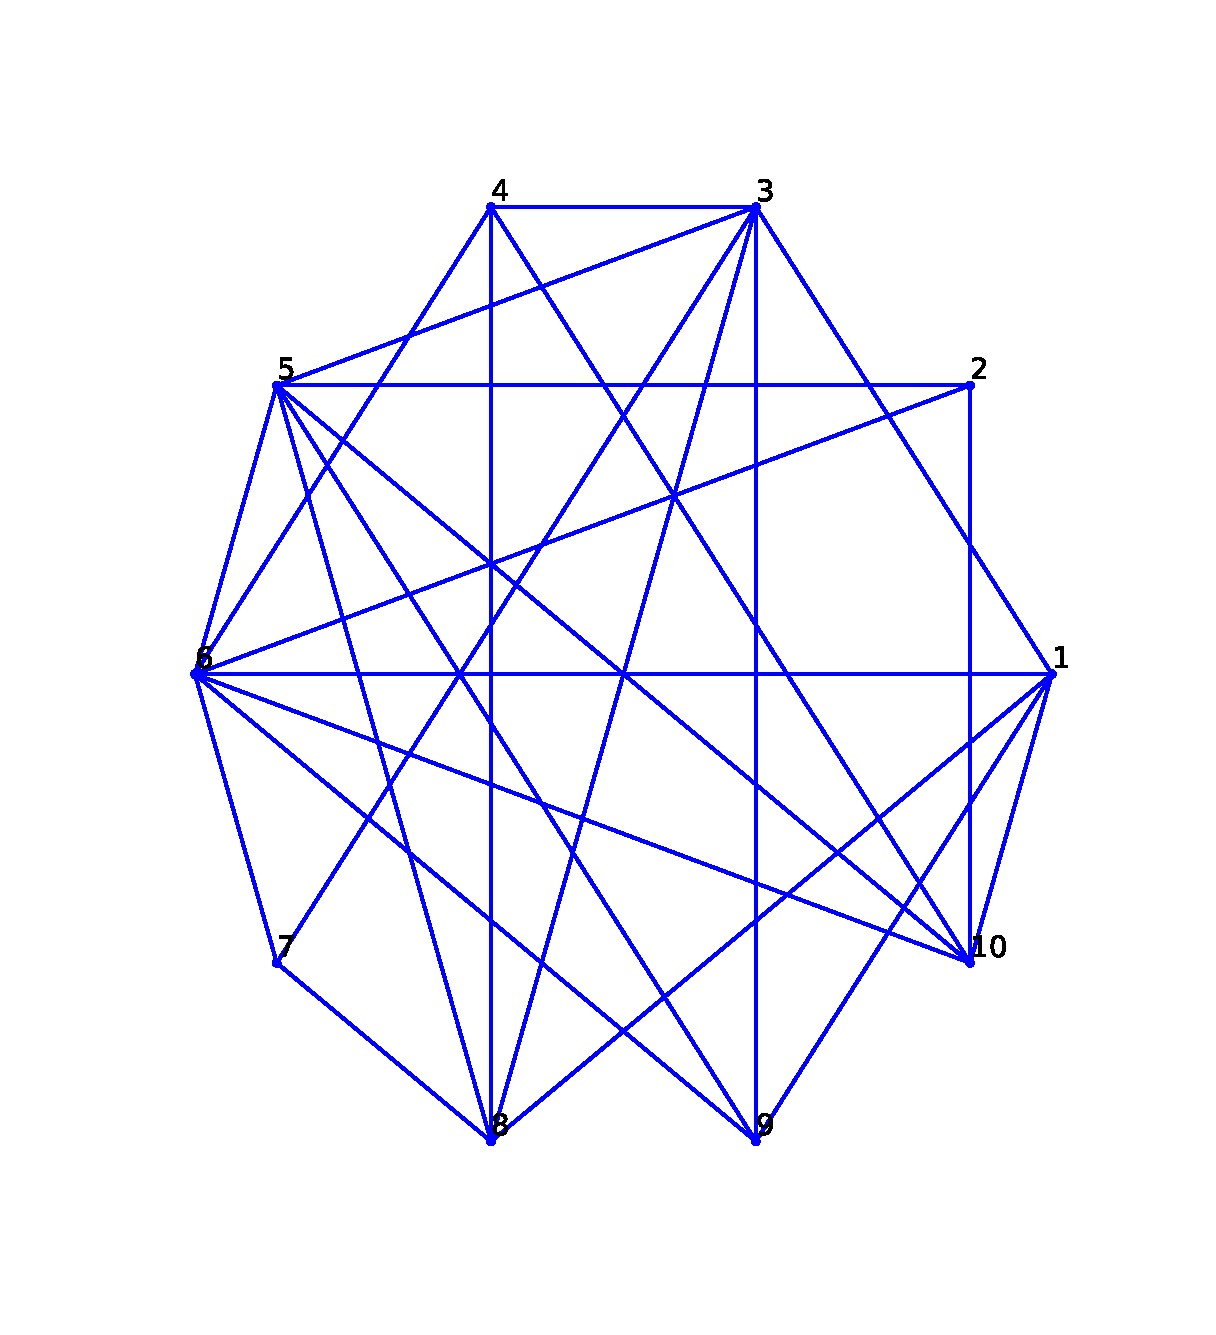
\includegraphics[scale=0.5]{g1.pdf}
    \caption{Пример диаграммы графа.}
    \label{gexp_1}
\end{figure} 
\begin{figure}[H] 
    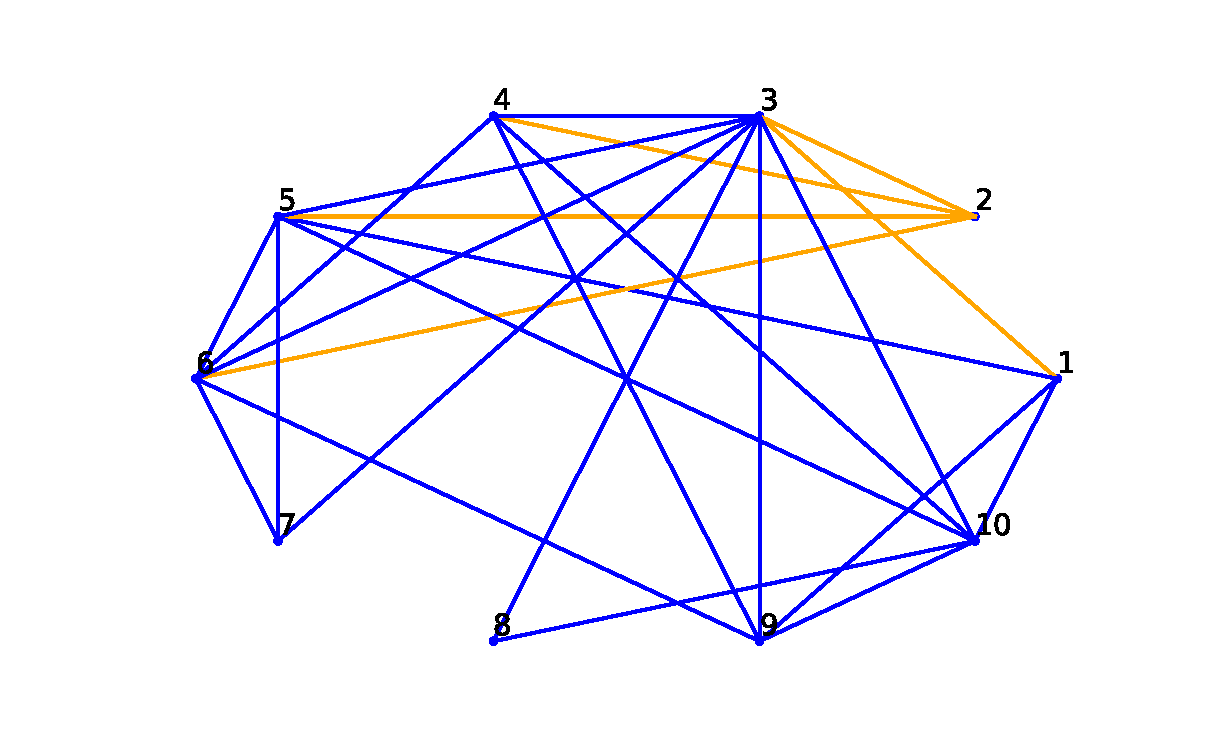
\includegraphics[scale=0.5]{g2.pdf}
    \caption{Пример диаграммы графа с оранжевыми ребрами.}
    \label{gexp_2}
\end{figure} 
На рисунках \ref{gexp_1}, \ref{gexp_2}
представлены диаграммы графов, созданные с помощью
<<GraphPlotter>>.

\section{ГЕНЕРАЦИЯ СЛУЧАЙНЫХ ГРАФОВ}
Для многих задач требуется генерация 
случайного графа. Будут рассмотрены 
разные модели генерации случайного графа \cite{rnd}. Каждая 
модель представлена отдельным модулем.
\subsection{Модель Эрдеша-Ренье}
Рассмотрим простейшую модель генерации случайного графа. 
Даны $n \in \mathbb{N}, p \in (0,1)$. Создается 
полный граф с $n$ вершинами, каждое
ребро берется с вероятностью  $p$.

\begin{figure}[H] 
\begin{lstlisting}[language=Python] 
    def complete_graph_edges(k):
        edges = []
        for a in range(1, k+1):
            for b in range(a+1, k+1):
                edges.append((a, b))
                edges.append((b, a))
        return edges
\end{lstlisting}  
\caption{Генерация списка ребер полного графа с
$k$ вершинами}
\label{erd_1}
\end{figure}
\begin{figure}[H] 
\begin{lstlisting}[language=Python] 
    def erdos_renyi_random_graph(n, p):
        edges = [e for e in ErdosRenyiGraph.complete_graph_edges(
            n) if random() < p]
        g = Graph()
        g.add_edges(edges)
        g.add_vertecies(range(1, n+1))
        return g
\end{lstlisting}  
\caption{Генерация случайного графа по модели Эрдеша-Ренье }
\label{erd_2}
\end{figure} 
На рисунках \ref{erd_1},\ref{erd_2}
приведен код для генерация случайного графа.
\begin{figure}[H] 
    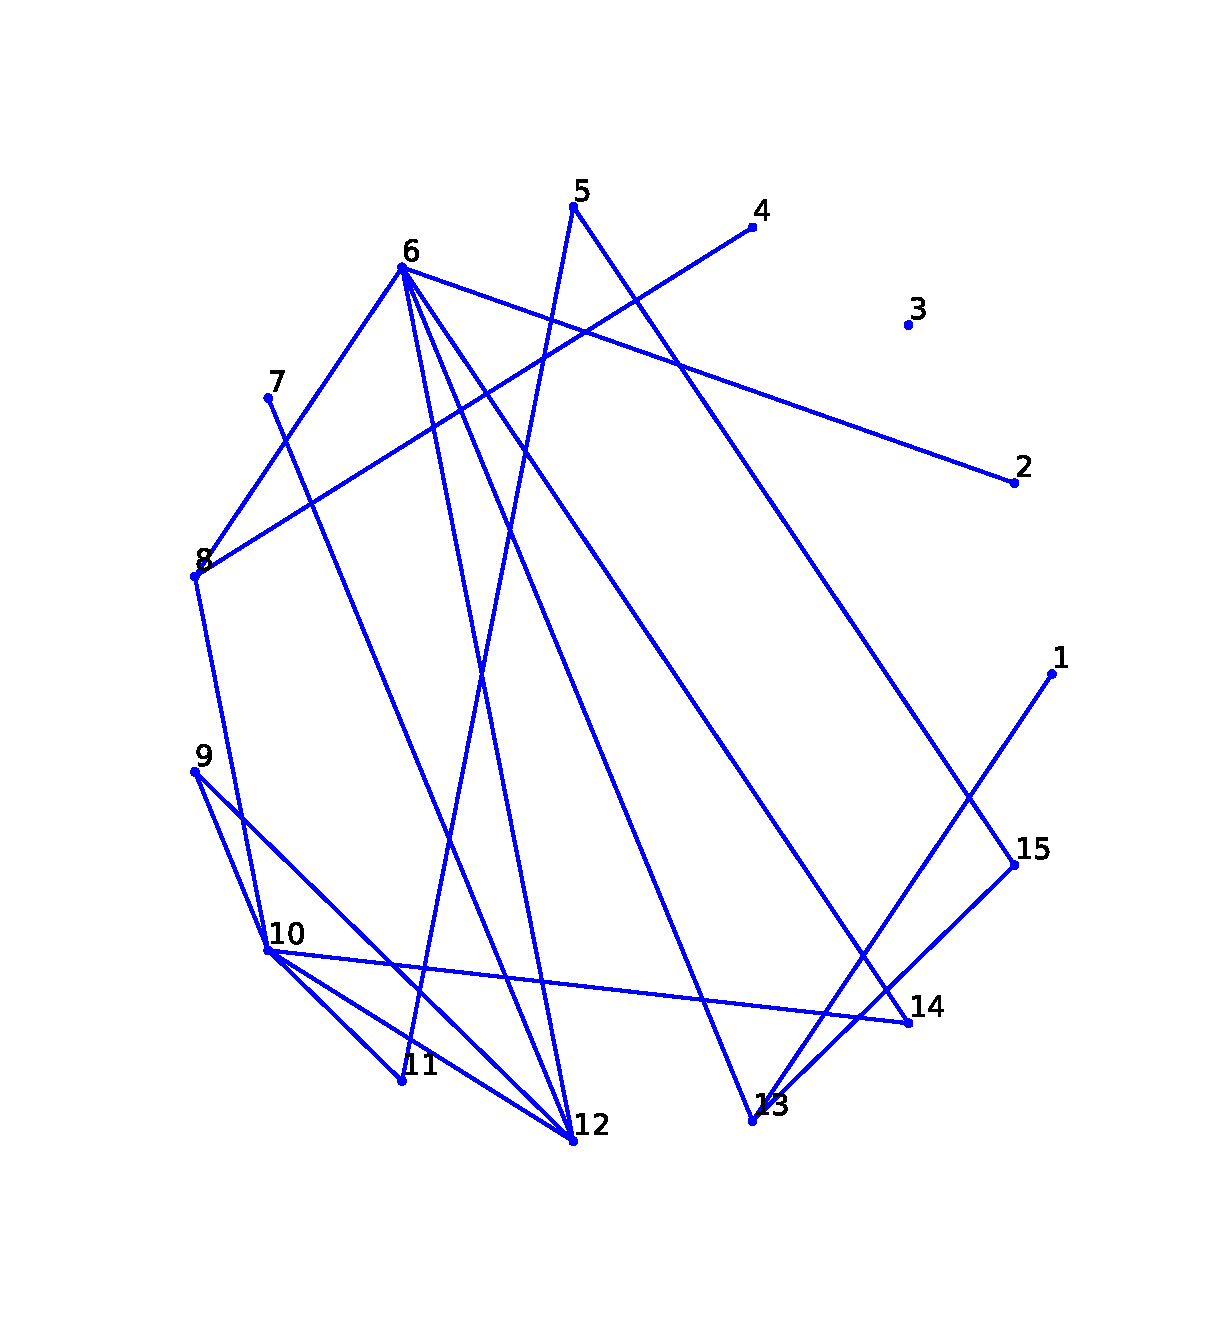
\includegraphics[scale=0.5]{erd1.pdf} 
    \caption{Случайный граф созданный с помощью модели Эрдеша-Ренье с
    параметрами $n = 15, p = 0.1$}
    \label{erd_3}
\end{figure} 
\begin{figure}[H] 
    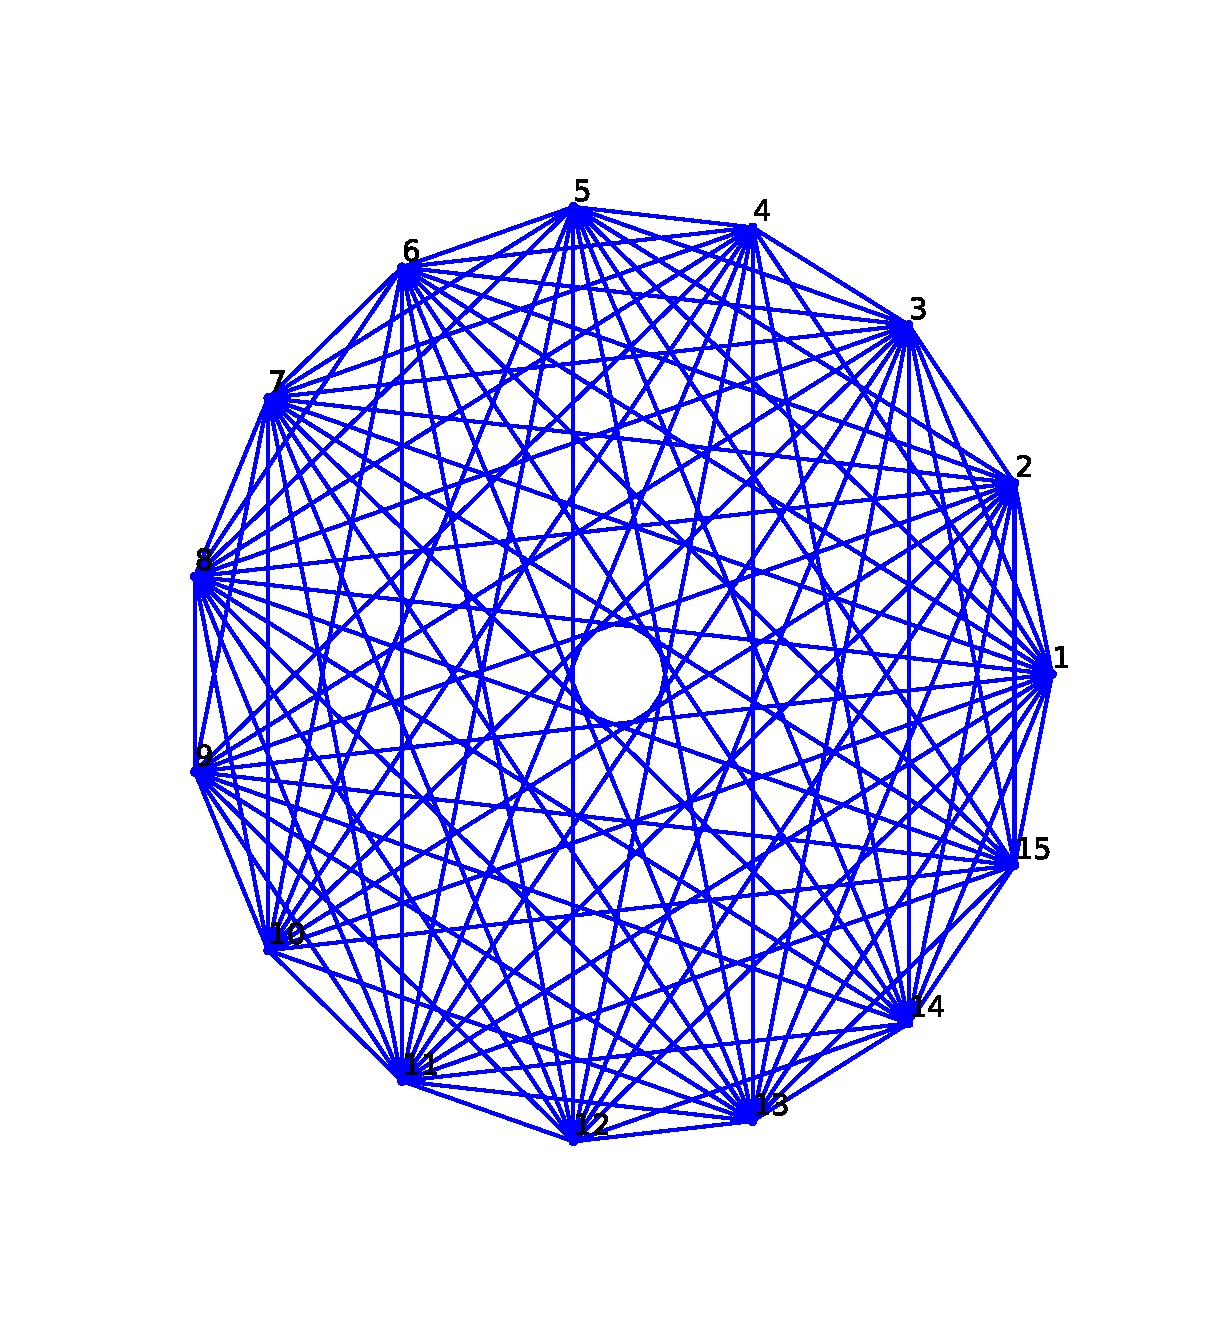
\includegraphics[scale=0.5]{erd2.pdf}
    \caption{Случайный граф созданный с помощью модели Эрдеша-Ренье с
    параметрами $n = 15, p = 0.7$}
    \label{erd_4}
\end{figure} 
На рисунках \ref{erd_3}, \ref{erd_4}
приведены примеры графов, созданных с помощью
данной модели. 

Графы созданные с помощью модели Эрдеша-Ренье плохо
описывают реальные сетевые структуры такие, как 
социальные сети. 
\subsection{Модель Барабаши-Альберт}
Пусть дан граф с $n$ вершинами и  $m \le n \in \mathbb{N}$.
Будем добавлять вершины пошагово, 
каждая добавленная вершина должна 
иметь $m$ ребер. 
 \begin{equation}
     P_{in} = \frac{\deg{i}}{ \sum_{j} \deg{j}}
     \label{ba}
\end{equation} 
Формула \ref{ba} обозначает вероятность добавления ребра
$\{i,n\}$
\begin{figure}[H] 
\begin{lstlisting}[language=Python] 
    def add_vertex(self, vertex):
        if vertex not in self.graph.verticies():
            total_deg = sum(self.graph.deg(v) for v in self.graph.verticies())
            p = [self.graph.deg(v) / total_deg for v in self.graph.verticies()]
            end = choice(list(self.graph.verticies()),
                         p=p, size=self.m, replace=False)
            for v1 in end:
                self.graph.add_edge(vertex, v1)
\end{lstlisting}  
    \caption{Реализация добавления вершины согласно модели Барабаши-Альберт}
    \label{ba_1}
\end{figure} 
На рисунке \ref{ba_1} приведен код, который реализует 
добавление новой вершины в граф, согласно данной модели.
\begin{figure}[H] 
    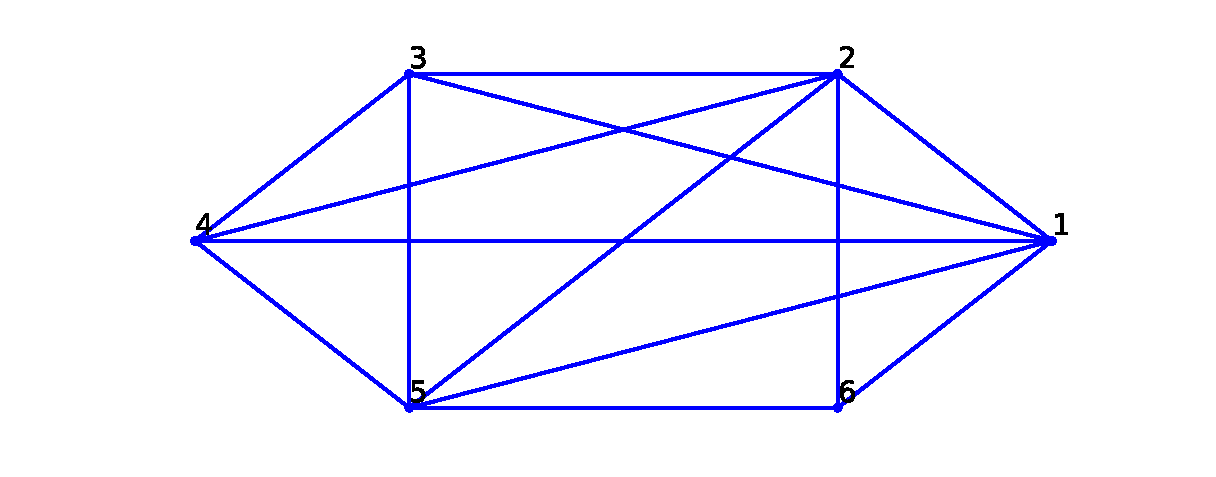
\includegraphics[scale=0.4]{ba1.pdf} 
    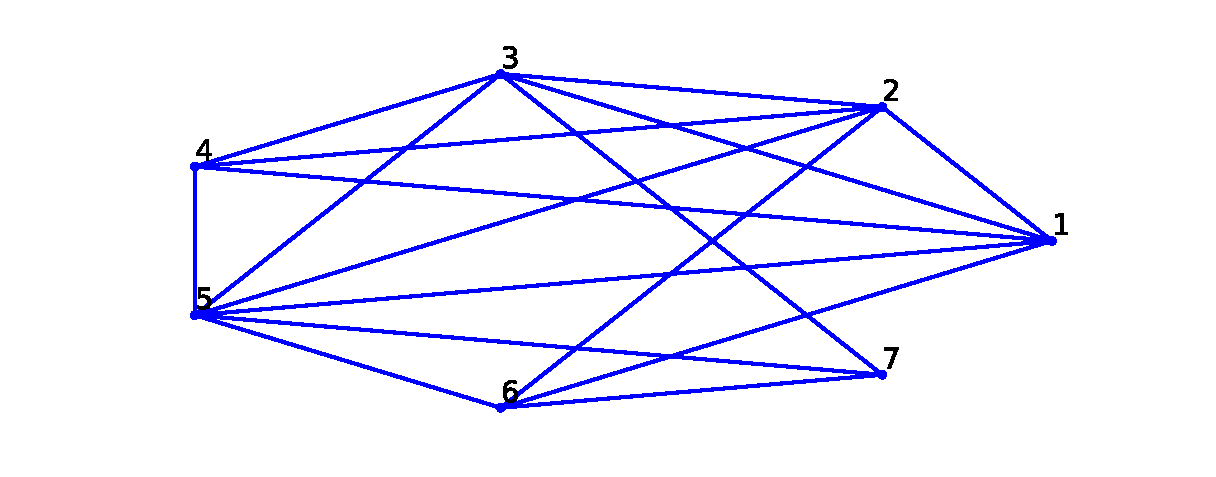
\includegraphics[scale=0.4]{ba2.pdf} 
    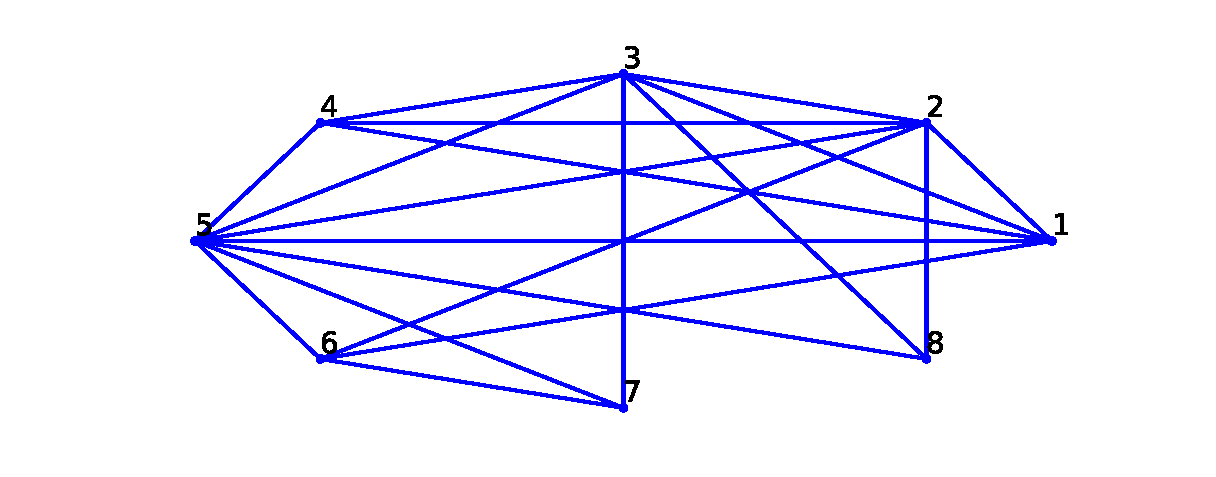
\includegraphics[scale=0.4]{ba3.pdf} 
    \caption{Визуализация построения 
    случайного графа с помощью модели Барабаши-Альберт с параметрами
$n=5,m=3$}
\label{ba_4}
\end{figure} 
На рисунке \ref{ba_4} приведны три шага итерации построения
случайного графа, согласно модели Барабаши-Альберт.
\subsection{Модель Боллобаша-Риордана}
Пусть дан граф с одной вершиной и петлей. 
Добавляем пошагово вершины. Пусть граф с $n-1$ 
вершиной построен, тогда 
$P_{in} = \frac{\deg{i}}{2n - 1}$, $P_{nn} = \frac{1}{2n - 1}$
\begin{figure}[H] 
\begin{lstlisting}[language=Python] 
    def __init__(self, n):
        g = Graph()
        g.add_edge(1, 1)
        for v in range(2, n+1):
            p = [g.deg(vertex) / (2*n - 1) for vertex in g.verticies()]
            p.append(1 / (2*n - 1))
            g.add_vertex(v)
            end = choices(list(g.verticies()), weights=p, k=1)
            g.add_edge(v, end[0])
        self.graph = g
\end{lstlisting}  
    \caption{Построение графа с $n$ вершинами, согласно модели 
    Боллобаша-Риодана.}
    \label{br_1}
\end{figure} 
На рисунке \ref{br_1} приведен код для генерации случайного графа
c помощью модели Боллобаша-Риодана.
\begin{figure}[H] 
    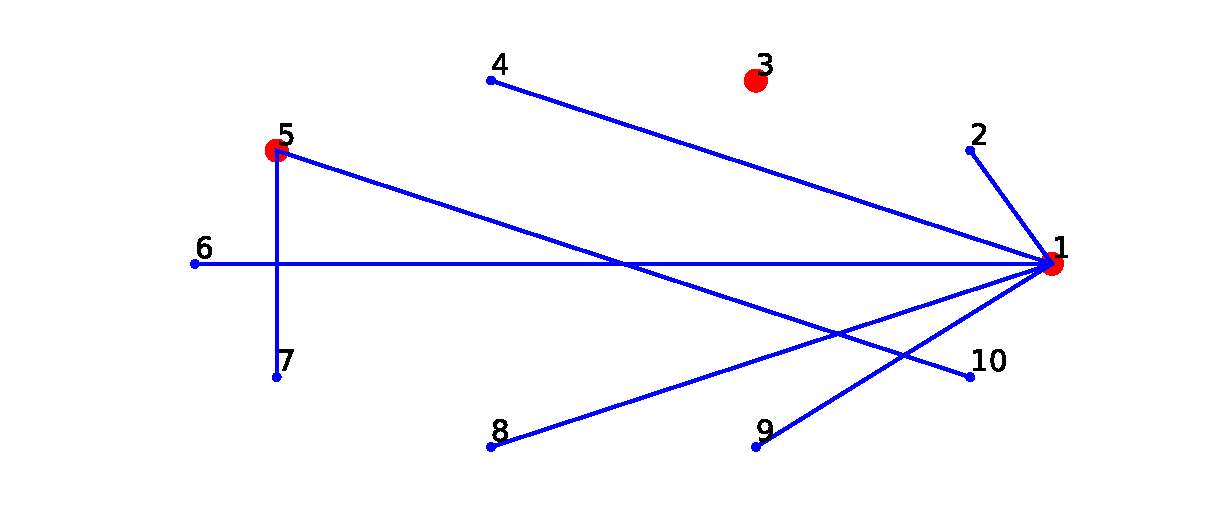
\includegraphics{br.pdf} 
    \caption{Граф с 10 вершинами, построенный согласно модели
    Боллобаша-Риодана}
    \label{br_2}
\end{figure} 
На рисунке \ref{br_2} изображен граф построенный согласно данной модели.
\subsection{Модель Боллобаша-Риодана для создания ориентированного графа}
Рассмотрим следущую модель генерации случайного ориентированного графа \cite{bolor}. Пусть даны неотрицательные вещественные числа 
$\alpha,\beta,\gamma,\delta_{\text{in}},\delta_{\text{out}}$, где
$\alpha + \beta + \gamma = 1$ и ориентированный граф  $G(1)$.
Будет создаваться последовательность $G(1),G(2),\dots, G(t),G(t+1) \dots G(n)$, где следущий граф строится по предыдущему.
Пусть вершина  $v \in V(t)$ выбирается согласно $d_{\text{in}} + \delta_{\text{in}}$, если 
вероятность выбора этой вершин из $V(t)$ равна  $\frac{d_{\text{in}}(v) +\delta_{\text{in}}}{t + \delta_{\text{in}} \cdot |V(t)|}$,
выбирается согласно $d_{\text{out}} + \delta_{\text{out}}$ 
если вероятность выбора данной вершины из $V(t)$ равна 
$\frac{d_{\text{out}}(v) +\delta_{\text{out}}}{t + \delta_{\text{out}} \cdot |V(t)|}$, где $d_{\text{in}}(v)$ -- полустепень захода вершины $v$, $d_{\text{out}}(v)$ -- полустепень исхода вершины $v$.

Граф $G(t+1)$ строится согласно следущему правилу:
 \begin{enumerate}
    \item с вероятностью $\alpha$ добавляется ребро  $(v,w)$,
        где  $v$ новая вершина,  $w$ вершина выбранная согласно  $d_{\text{in}} + \delta_{\text{out}}$ ;
    \item с вероятностью $\beta$ добавляется ребро  $(v,w)$,
        где вершина  $v$ добавляется согласно  $d_{\text{out}} + \delta_{\text{out}}$, вершина $w$ выбирается согласно  $d_{\text{in}} + \delta_{\text{in}}$;
     \item с вероятностью $\gamma$ добавляется ребро  $(v,w)$,
         где  $v$ новая вершина,  $w$ выбирается согласно 
         $d_{\text{out}} + \delta_{\text{out}}$ ;
\end{enumerate}
Рассмотрим реализацию данного алгоритма.
\begin{figure}[H] 
\begin{lstlisting}[language=Python] 
    def d_in_p(self, v):
        return (self.graph.in_deg(v) + self.d_in) / (self.t + self.d_in * self.graph.k_vertecies())

    def d_out_p(self, v):
        return (self.graph.out_deg(v) + self.d_in) / (self.t + self.d_out * self.graph.k_vertecies())

    def rnd_in(self):
        probs_in = [self.d_in_p(v) for v in self.graph.verticies()]
        return choices(list(self.graph.verticies()),
                       weights=probs_in, k=1)[0]

    def rnd_out(self):
        probs_out = [self.d_out_p(v) for v in self.graph.verticies()]
        return choices(list(self.graph.verticies()),
                       weights=probs_out, k=1)[0]
\end{lstlisting}  
    \caption{Получение случайных вершин графа}
    \label{orrnd_1}
\end{figure} 
На рисунке \ref{orrnd_1} приведен код для получения вершин 
графа согласно $d_{\text{in}} + \delta_{\text{in}}$ и $d_{\text{out}} +
\delta_{\text{out}}$
\begin{figure}[H] 
\begin{lstlisting}[language=Python] 
    def add_vertex(self):
        p = random()
        if p < self.alpha:
            v = self.nxt
            self.nxt += 1
            w = self.rnd_in()
            self.graph.add_edge(v, w)
        if p < self.beta:
            v = self.rnd_in()
            w = self.rnd_out()
            self.graph.add_edge(v, w)
        if p < self.gamma:
            w = self.nxt
            self.nxt += 1
            v = self.rnd_out()
            self.graph.add_edge(v, w)
        self.t += 1
\end{lstlisting}  
    \caption{Добавление вершины в граф согласно данной модели}
    \label{orrnd_2}
\end{figure} 
На рисунке \ref{orrnd_2} приведена реализация добавления вершины 
в ориентированный граф.
\begin{figure}[H] 
    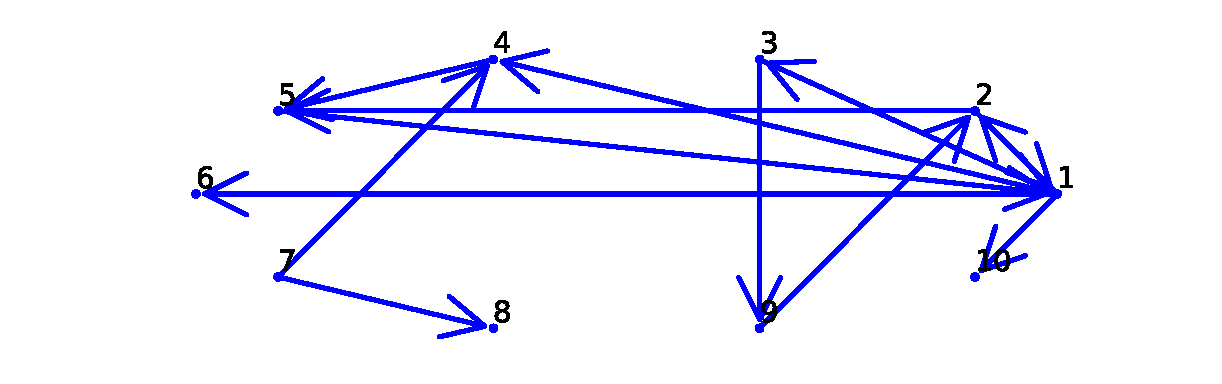
\includegraphics{or1.pdf} 
    \caption{Пример графа созданного с помощью данной модели}
    \label{orrnd_3}
\end{figure} 
На рисунке \ref{orrnd_3} приведена диаграмма графа созданного с помощью данной модели,
где $\alpha = 0.4,\beta = 0.4,\gamma =0.2, \delta_{\text{in}} = 2, \delta_{\text{out}} = 2$.
\subsection{Модель Бакли-Остхус}
Рассмотрим следущую \cite{buck} модификацию модели Боллобаша-Риодана. 
Дан граф с одной вершиной и петлей и параметр $a$. 
На  $i+1$-том шаге  вершина $i+1$ добавляется в граф, из нее 
проводится ребро в случайную вершину, которая выбирается со следушей вероятностью $P_{k,i+1} = \frac{\deg{k} + a }{(a+1)*(i+1) - 1}$,
$P_{i+1,i+1} = \frac{a}{(a+1)(i+1) - 1}$.

Рассмотрим реализацию данной модели.
\begin{figure}[H] 
\begin{lstlisting}[language=Python] 
    def add_edge(self):
        p = [(self.graph.deg(v) + self.a) / ((self.a+1) *
                                             (self.graph.k_vertecies() + 1) - 1) for v in self.graph.verticies()]
        p.append(self.a / ((self.a+1) * (self.graph.k_vertecies() + 1)-1))
        self.graph.add_vertex(self.nxt)
        v = choices(list(self.graph.verticies()), weights=p, k=1)[0]
        self.graph.add_edge(self.nxt, v)
        self.nxt += 1
\end{lstlisting}  
    \caption{Добавление вершины в граф}
    \label{os_1}
\end{figure} 
На риснуке \ref{os_1} представлен метод, реализующий добавление 
вершины в граф, согласно модели Бакли-Остхус.
\begin{figure}[H] 
    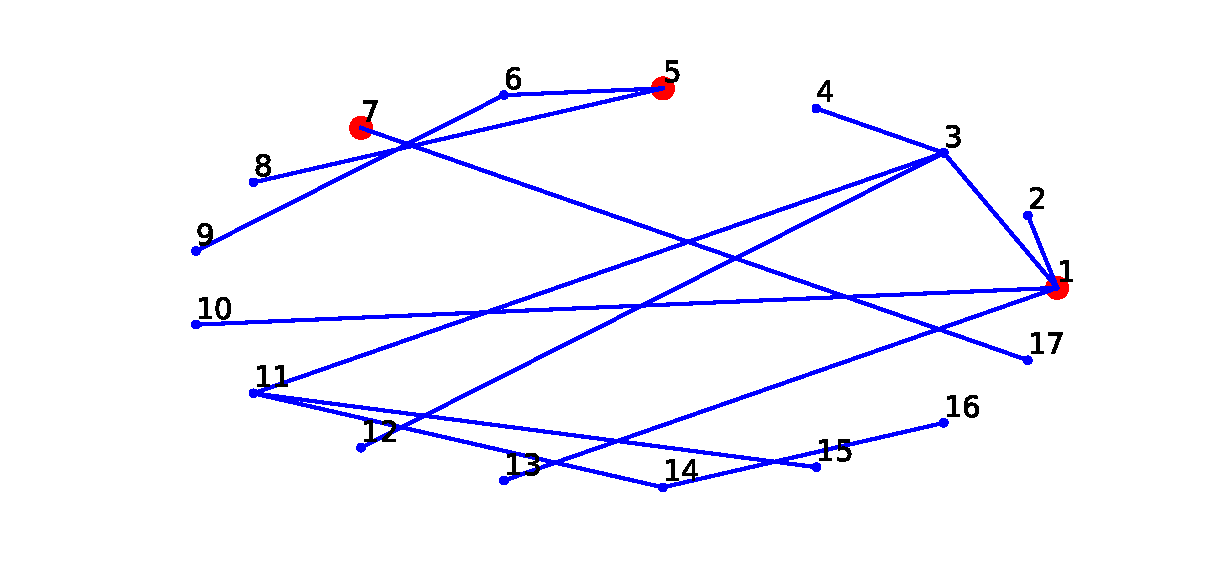
\includegraphics[scale=0.8]{os.pdf} 
    \caption{Пример графа, созданного с помощью модели Бакли-Остхус с параметром $a=2$}
    \label{os_2}
\end{figure} 
На рисунке \ref{os_2} представлен пример результата работы данной модели.
\subsection{Модель LCD}
Рассмотрим алгоритм генерации графа с помощью линейной хордовой
диаграммы (LCD):
\begin{enumerate}
    \item идем слева направо;
    \item добавляем в набор вершины, пока не встретим конец дуги;
    \item собранный набор становится вершиной графа, дуги становятся дугами графа;
\end{enumerate}
\begin{figure}[H] 
\begin{lstlisting}[language=Python] 
def __init__(self, n):
k = 2*n
    nums = list(range(1, k+1))
    self.left = []
    self.right = []
    for _ in range(n):
        l = choice(nums)
        nums.remove(l)
        r = choice(nums)
        nums.remove(r)
        self.left.append(l)
        self.right.append(r)
    v = []
    curr = []
    nums = list(range(1, k+1))
    for i in nums:
        curr.append(i)
        if i in self.right:
            v.append(curr.copy())
            curr = []
    g = Graph()
    for i, lst in enumerate(v, 1):
        g.add_vertex(i)
        for j, v2 in enumerate(lst):
            if v2 in self.left:
                r = self.right[j]
                for k in range(len(v)):
                    if r in v[k]:
                        g.add_edge(i, k+1)
    self.graph = g
\end{lstlisting}  
    \caption{Реализация LCD алгоритма.}
    \label{lcd1}
\end{figure} 
На рисунке \ref{lcd1} приведена реализация 
LCD алгоритма
\begin{figure}[H] 
    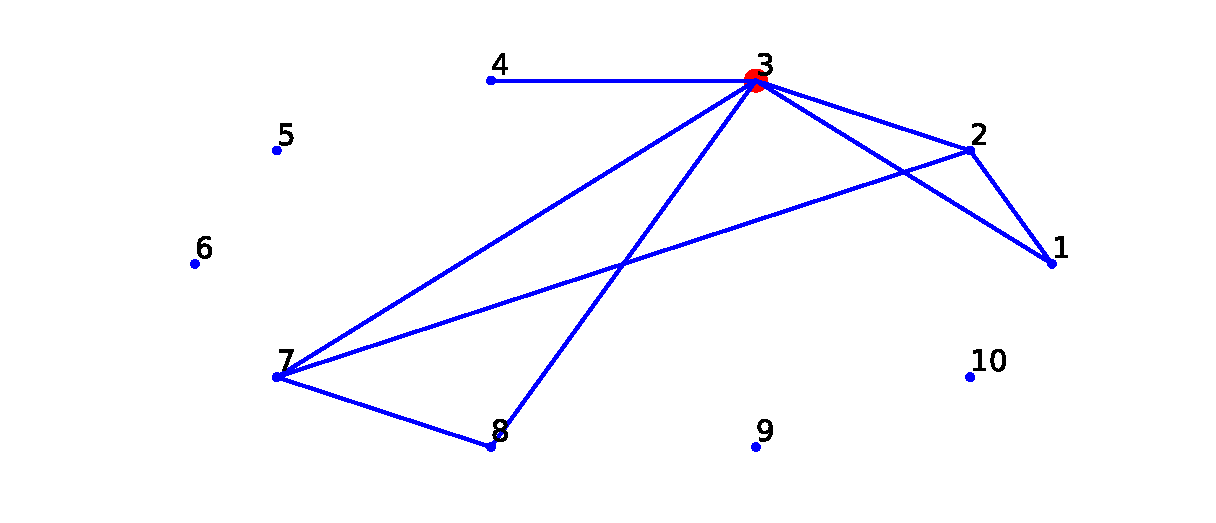
\includegraphics{lcd.pdf} 
    \caption{Граф, созданный с помощью LCD алгоритма}
    \label{lcd2}
\end{figure} 
На рисунке \ref{lcd2} приведен пример графа, созданного с помощью 
данного алгоритма.
\subsection{Модель копирования}
Пусть даны $\alpha \in (0,1)$ и 
 d-регулярный граф $d \ge  1$ , $V$ -- множество вершин этого графа. Рассмотрим алгоритм добавления вершины в граф:
 \begin{enumerate}
     \item выберем случайную вершину $p \in V$;
     \item добавляем d вершин по следущему правилу:
         с вероятностью $\alpha$ строим ребро из новой вершины 
         в  $p$ , c вероятностью $1 - \alpha$ строим
         ребро из новой вершины в  $i$-го соседа вершины  $p$;
 \end{enumerate}
 \begin{figure}[H] 
 \begin{lstlisting}[language=Python] 
    def add_vertex(self):
        v = self.j + 1
        self.j+=1
        p = choice(self.start_verticies)
        for i in range(self.d):
            if random() < self.alpha:
                self.graph.add_edge(p, v)
            else:
                self.graph.add_edge(list(self.graph.neib(p))[i], v)
 \end{lstlisting}  
     \caption{Метод, реализующий алгоритм добавления вершин,
     согласно модели копирования.}
     \label{cop1}
 \end{figure} 
 На рисунке \ref{cop1} приведен метод 
добавления вершин в граф, согласно модели копирования.
\begin{figure}[H] 
    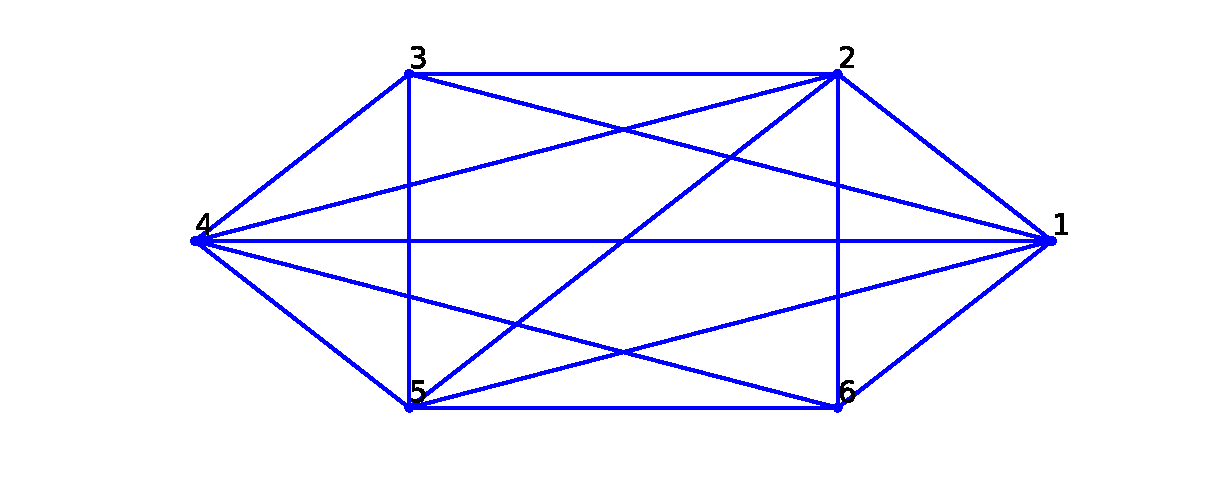
\includegraphics[scale=0.8]{cop1.pdf} 
    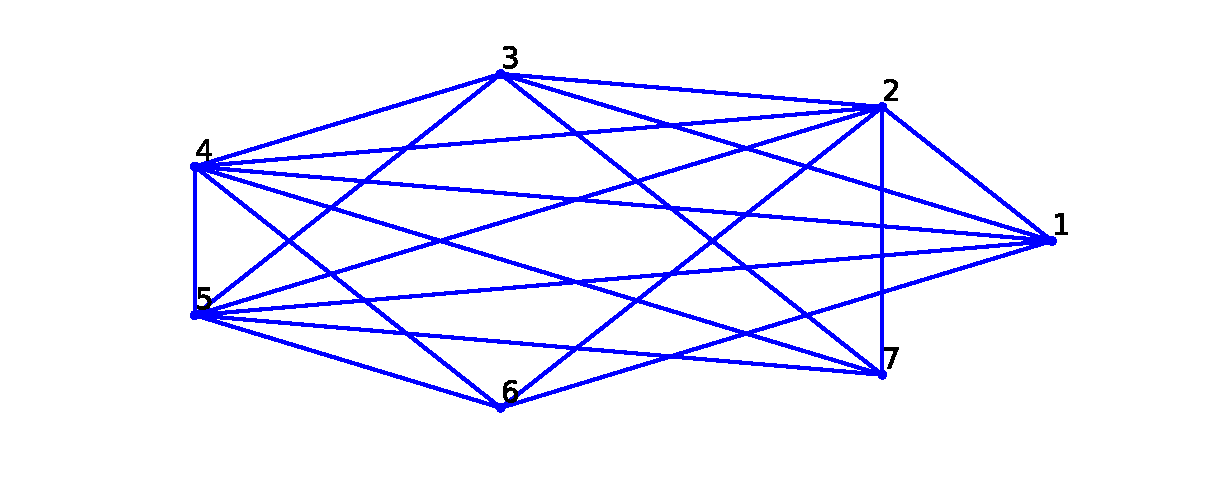
\includegraphics[scale=0.8]{cop2.pdf} 
    \caption{Результат добавления двух вершин в граф 
    с параметрами $d = 4,\alpha = 0.1$ согласно модели копирования.}
    \label{cop2}
\end{figure} 
На рисунке \ref{cop2} приведен пример генерации случайного графа согласно модели копирования.
\subsection{Модель Чунг-Ли}
Рассмотрим модель генерации случайного 
мультиграфа. Пусть нам дана степень каждой вершины,
степень $i$-ой вершины 
обозначим как  $d_{i}$. Граф генерируется следущим образом:
\begin{enumerate}
    \item строится множество $L$, которое состоит из
         $d_{i}$ копий вершины $i$;
    \item задаются случайные паросочетания на $L$;
    \item число парасочетаний между копиями  $u$ и  $v$ --
        число ребер между  $u$ и $v$;
\end{enumerate}
\begin{figure}[H] 
\begin{lstlisting}[language=Python] 
    def __init__(self, d: [int]):
        self.d = d
        self.l_set = []
        for i, elem in enumerate(d, 1):
            for _ in range(elem):
                self.l_set.append(i)

        self.edges = []
        for _ in range(sum(d)//2):
            a = choice(self.l_set)
            self.l_set.remove(a)
            b = choice(self.l_set)
            self.l_set.remove(b)
            self.edges.append((a, b))
        self.graph = MultiGraph()
\end{lstlisting}  
    \caption{Генерация случайного мультиграфа согласно модели ЧунгЛи.}
    \label{ch1}
\end{figure} 
На рисунке \ref{ch1} приведен код для создания случайного мультиграфа согласно данной модели.
\begin{figure}[H] 
    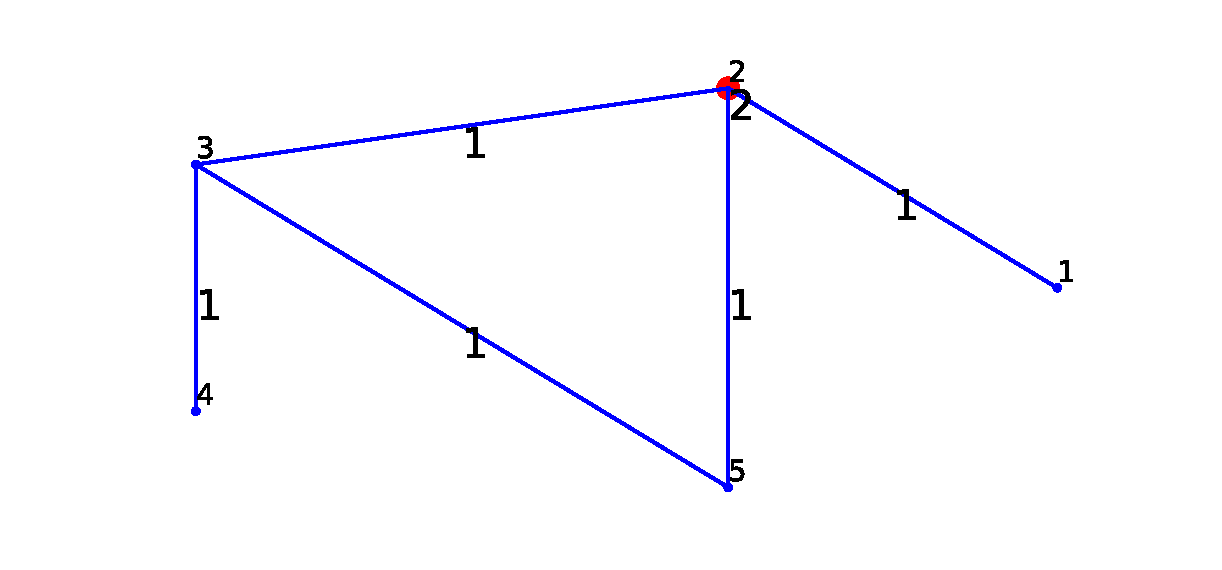
\includegraphics{ch.pdf}
    \caption{Мультиграф созданный с помощью модели Чунг-Ли,
    где $d = [1,5,2,1,2]$}
    \label{ch2}
\end{figure} 
Пример случайного мультиграфа, полученного согласно данно модели
приведен на рисунке \ref{ch2}.
\subsection{Модель Янсона-Лучака}
Рассмотрим набор вершин $v = \{v_1 \dots v_{n}\}$ и набор весов
$W = \{W_1 \dots W_{n}\}$.  Пусть
$\lambda_{ij} = \frac{W_{i} W_{j} }{n}$ -- математическое 
ожидание случайной величины $E_{ij}$, имеющей Пуассоновское распределение. Для вершин $i,j$ строится  $E_{ij}$ кратных ребер.
Получившийся мультиграф можно преобразовать в граф,
путем стягивания кратных ребер.
\begin{figure}[H] 
\begin{lstlisting}[language=Python] 
    def gen_graph(self):
        rng = np.random.default_rng()
        graph = MultiGraph()
        for (u, v) in combinations(range(1, len(self.weights)+1), 2):
            lamb = (self.weights[u-1]*self.weights[v-1]) / len(self.weights)
            for _ in range(int(lamb)):
                graph.add_edge(u,v)
            graph.add_vertecies((u,v))
        self.graph = graph
\end{lstlisting}  
    \caption{Генерация случайного графа согласно модели Янсона-Лучака.}
    \label{jason_1}
\end{figure} 
На рисунке \ref{jason_1} приведена реализация алгоритма 
создания случайного графа, согласно модели Янсона-Лучака.
Для генерации случайной величины используется библиотека <<numpy>> \cite{numpy}.
\begin{figure}[H] 
    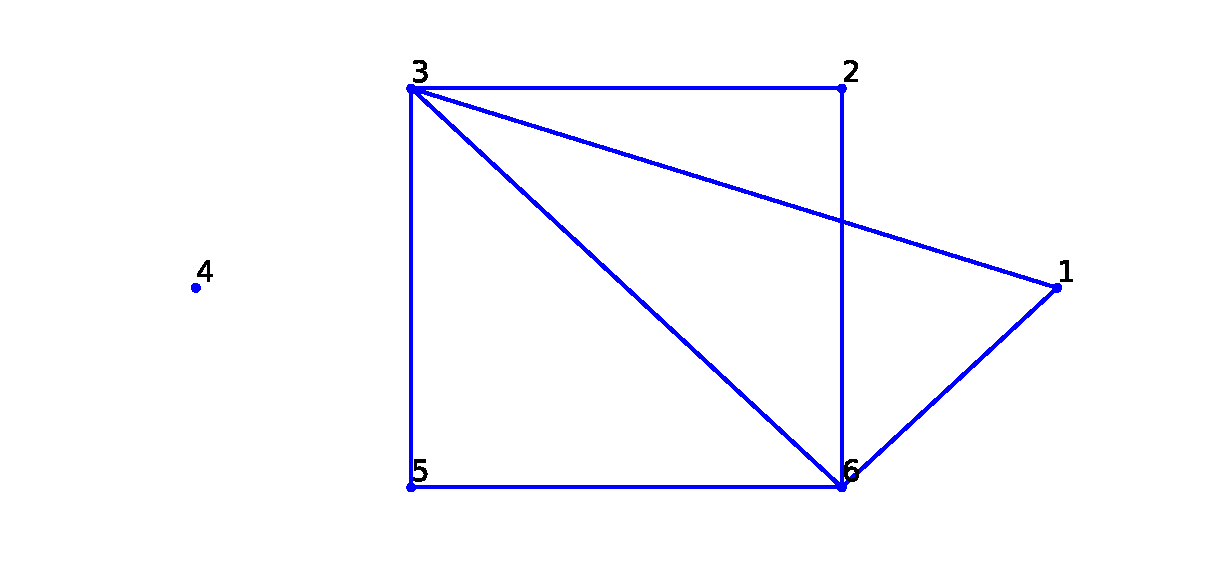
\includegraphics{jason.pdf} 
    \caption{Пример графа, созданного согласно модели Янсона-Лучака}
    \label{jason_2}
\end{figure} 
На рисунке \ref{jason_2} изображен граф, который был создан с 
помощью модели Янсона-Лучака, $w = \{2,2,3,1,3,2\} $.
\subsection{Генерация случайного геометрического графа}
Назовем граф $G(n,R)$ случайным геометрическим 
графом, если он получен путем размещения
на плоскости  $n$ вершин и две вершины
инцидентны, если евклидово расстояние между ними не превышает  $R$.
\subsubsection{Эффективный алгоритм генерации геометрических графов.}

 Пусть на 
плоскость наложена сетка, состоящая из 
квадратных ячеек с шагом  $\frac{R}{\sqrt{2} }$. Обозначим 
ячейку  $i$-тую по вертикали и  $j$-тую по вертикали как $L_{ij}$,
всего ячеек $L_{\text{size}}^2$. Назовем множество 
$\Omega_{ij} = \{(L_{kl} \mid  k \in -2 \dots 2, n \in -2 \dots 2 , 
0 \le  |k| + |m| < 3\}$ псевдоокрестностью $L_{ij}$
Рассмотрим следущий алгоритм генерации случайных
геометрических графов \cite{geo} :
\begin{enumerate}
    \item в каждой ячейке создается случайная вершина;
    \item для $i,j$ вершины создаются ребра смежные
        вершинам из  $\Omega_{ij}$, если расстояние между ними не превышает $R$;
    \item  $n_{\text{curr}} = n - L^2_{\text{size}}$ -- число несгенированных вершин;
    \item $N = n - L^2_{\text{size}}$ ;
    \item $p = \frac{1}{L^2_{\text{size}}}$ ;
    \item для $L_{ij}$ вычисляется $s_{ij} = \min(n_{\text{curr},B(N,p)})$, где $B(N,p)$ случайная величина распределенная по 
        биноминальному закону;
    \item в $L_{ij}$ создается $s_{ij}$ вершин;
    \item каждая созданная вершина соединяется с вершинами из
        $\Omega_{ij}$, если расстояние не превышает $R$;
    \item  $n_{\text{ curr }}$ уменьшается на $s_{ij}$ ;
    \item если $n_{\text{curr}} = 0$ то граф построен;
\end{enumerate}
Данный алгоритм является достаточно эффективным и
создает графы похожие на реальные структуры, такие 
как беспроводные сети.
\subsubsection{Реализация алгоритма генерации геометрических графов}
Геометрический граф будет реализован с 
помощью класса <<GeoGraph>>, который 
является потомком класса <<Graph>>. Для
реализации веришн был реализован класс <<Node>>, имеющий следущие
поля и методы:
\begin{enumerate}
    \item поле <<x>> -- координата по оси  $X$;
    \item  поле  <<y>> -- координата по оси $Y$;
    \item метод  <<dist>> -- вычисляет евклидово расстояние между 
        двумя вершинами;
\end{enumerate}
Рассмотрим реализацию на языке программирования Python.

\begin{figure}[H] 
\begin{lstlisting}[language=Python] 
@dataclass(frozen=True)
class Node:
    x: float
    y: float
\end{lstlisting}  
    \caption{Определение класса <<Node>>}
    \label{pynode_1}
\end{figure} 
\begin{figure}[H] 
\begin{lstlisting}[language=Python] 
    def dist(self, other):
        return sqrt((self.x - other.x) ** 2 + (self.y - other.y)**2)
\end{lstlisting}  
    \caption{Метод для вычисления еклидового расстояния между двумя вершинами.}
    \label{pynode_2}
\end{figure} 
На рисунках \ref{pynode_1}, \ref{pynode_2} приведена реализация вершины 
геометричесого графа.

Модель генерации случайного геометрического графа была 
определена в классе <<GeoGraphRndModel>>. В данном 
классе был определен метод инициализации и метод создания графа.
\begin{figure}[H] 
\begin{lstlisting}[language=Python] 
    def __init__(self, r, n):
        self.n = n
        self.r = r
        self.l_step = r/(sqrt(2))
        self.l_size = int(sqrt(n))
        self.grid = Grid(self.l_size)
        self.gen_graph()
\end{lstlisting}  
    \caption{Инициалиация модели генерации случайного геометрического графа.}
    \label{geornd1}
\end{figure} 
На рисунке \ref{geornd1} приведен метод создания 
модели случайного геометрического графа. Рассмотрим
реализацию алгоритма генерации случайного графа.
\begin{figure}[H] 
\begin{lstlisting}[language=Python] 
    def gen_graph(self):
        self.graph = GeoGraph()
        for lst in self.grid.grid.values():
            self.graph.add_vertecies(lst)
        for i in range(self.l_size):
            for j in range(self.l_size):
                for n1 in self.grid.grid[i, j]:
                    omega = self.grid.omega(i, j)
                    for n2 in omega:
                        if n1.dist(n2) <= self.r and n2 != n1:
                            self.graph.add_edge(n1, n2)
        N = self.n - self.l_size**2
        p = (1/self.l_size)**2
        n_curr = self.n - self.l_size**2
        for i in range(self.l_size):
            for j in range(self.l_size):
                s = binomial(N, p)
                s = min(s, n_curr)
                for _ in range(s):
                    n = Node(i+random(), j+random())
                    for n2 in self.grid.grid[i, j]:
                        self.graph.add_edge(n, n2)
                    omega = self.grid.omega(i, j)
                    for n2 in omega:
                        if n.dist(n2) <= self.r:
                            self.graph.add_edge(n, n2)
                    self.grid.grid[i, j].append(n)
                    self.graph.add_vertex(n)
                n_curr -= s
                if n_curr <= 0:
                    break
\end{lstlisting}  
    \caption{Реализация алгоритма генерации случайного геометрического
    графа}
    \label{geornd2}
\end{figure} 
На рисунке \ref{geornd2} приведен метод, 
реализующий генерацию случайного геометрического графа.

Рассмотрим примеры графов, созданных с помощью данного алгоритма.
\begin{figure}[H] 
    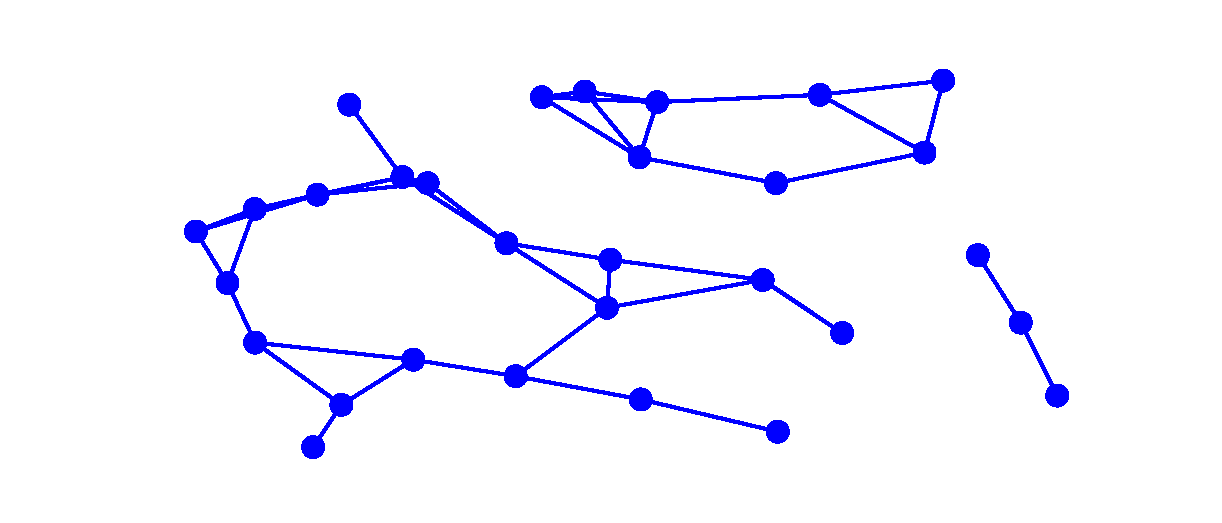
\includegraphics{geo301.pdf} 
    \caption{Случайный геометрический граф, $n=30$,  $R=1$}
    \label{geoex_1}
\end{figure} 
\begin{figure}[H] 
    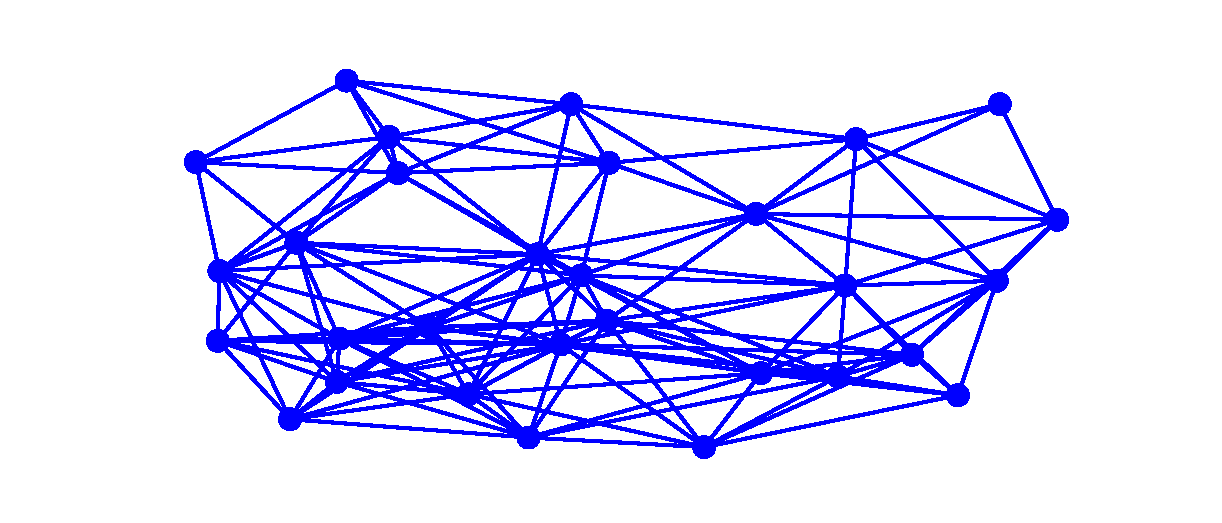
\includegraphics{geo302.pdf} 
    \caption{Случанйый геометрический граф, $n=30$,  $R=2$}
    \label{geoex_2}
\end{figure} 
На рисунках \ref{geoex_1},\ref{geoex_2} приведены 
примеры графов, созданных c помощью алгоритма генерации
случайных геометрических графов.

\end{document}
